\documentclass[conference]{IEEEtran} % Usa la classe IEEEtran per formattazione simile

\usepackage{amsmath}
\usepackage{graphicx}



\begin{document}

\title{Exploring the Adversarial Robustness of AI-generated Image Detectors}

\author{
    \IEEEauthorblockN{Thomas Lazzerini, Samuele Cappelletti, Martina D'Angelo}
    \IEEEauthorblockA{
        University of Trento
    }
}

\maketitle

\begin{abstract}
Semi-supervised image classification is a machine-learning task in which a model is trained using a combination of labeled and unlabeled data. This paper consists of a high-level survey of semi-supervised image classification literature and expands on its main theoretical and practical challenges, providing a taxonomy of the most popular semi-supervised learning algorithms. ciao come va
\end{abstract}

\section{Introduction}
Semi-supervised image classification is nowadays a hot research topic. The objective is to tackle the major issue of Supervised Learning: the scarcity of labeled data...
% Continua con il tuo contenuto

As discussed in \cite{corvi2023detection}, semi-supervised learning is an important area of research.

\begin{figure}[h]
    \centering
    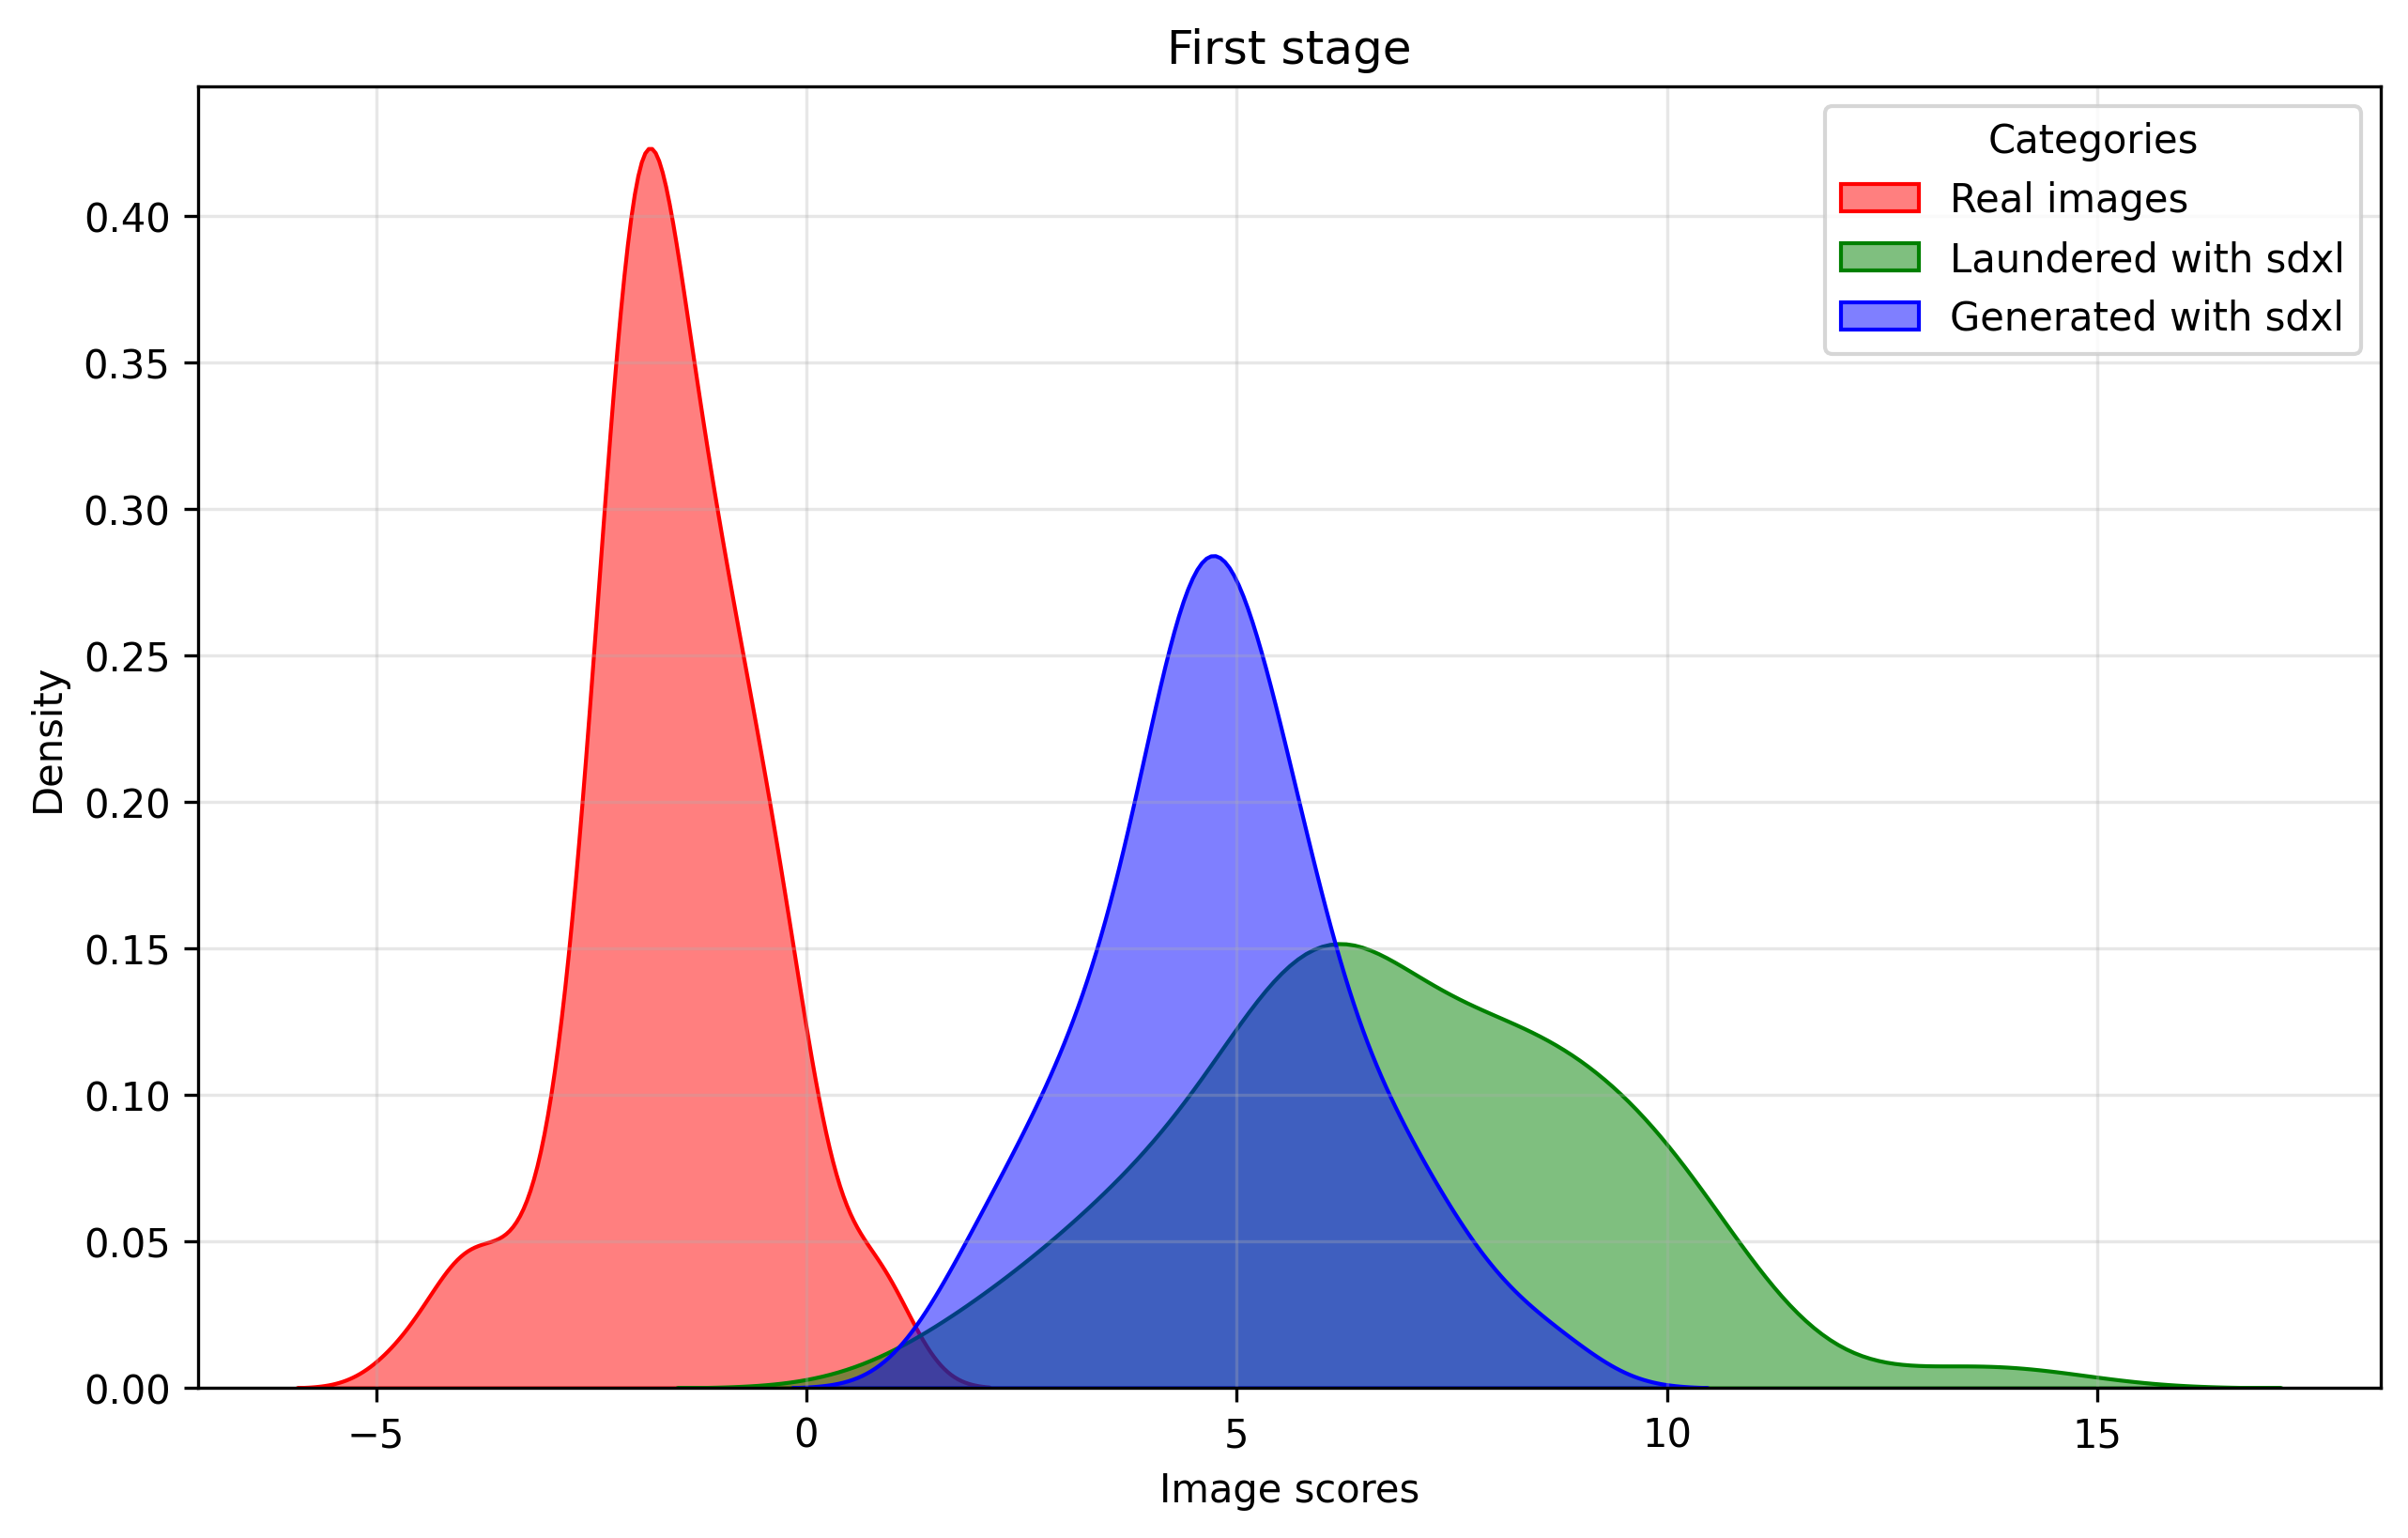
\includegraphics[width=0.8\linewidth]{Img/First_stage.png}
    \caption{Esempio di immagine.}
    \label{fig:esempio}
\end{figure}


\section{Detectors}
    \subsection{CLIP}
    \subsection{Detection of Images by Diffusion Models} 
        Lately, \textit{Diffusion Models} gained the spotlight in the image generation community, allowing for unmatched test-to-image photorealism and diversity. These new powerful tools are a new asset in the hands of malicious users, posing new challenges to the forensic community. 

        Most SoTA detectors exploits low-level artifacts, not visible by a human eye, introduced during the generation phase by GAN generators. The study in \cite{corvi2023detection} suggests that, as can be seen in Fig. \ref{fig:pizza_fourier}, similar traces can be found also in DM-generated images

        \begin{figure}[h]
            \centering
            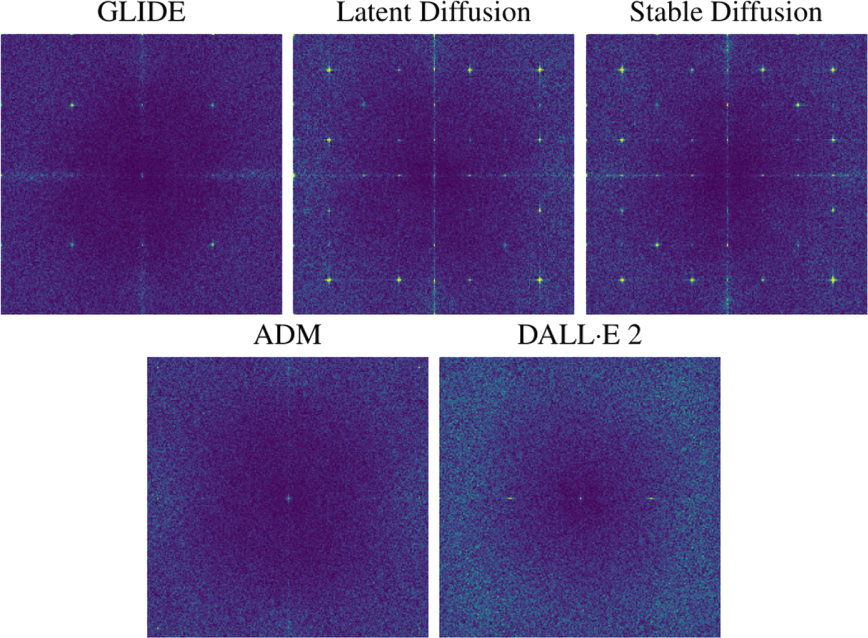
\includegraphics[width=0.8\linewidth]{Img/pizza_fourier.png}
            \caption{Fourier transform of of the fingerprint of some DM presented in \cite{corvi2023detection}}
            \label{fig:pizza_fourier}
        \end{figure}

        The study in \cite{corvi2023detection} also provides interesting evaluation results, comparing the performances of several SoTA detectors over different GAN and DM generators both in ideal case (uncompressed images) and real case (compressed and resized using the guidelines in \cite{vipcuplink}). These evaluations highlight how performances vary significantly between the models, due to the differences in their artifacts, therefore suggesting generalization difficulties (for example, in classifying a DM images with a GAN training and vice versa). Despite these difficulties, the inclusion of DM during training and performing an careful calibration procedure, like the one suggested by \cite{Platt1999probabilistic}, may help the generalization over similar architectures, despite not providing reliable results on out-of-training artifacts.
\section{Attacks}
    \subsection{Mimicry}
    \subsection{SD Laundering}
    \subsection{White Black}
    \subsection{Adversarial Robustness}
\section{Experiment}
\section{Conclusions}

\bibliographystyle{IEEEtran} % Stile delle referenze (es. IEEE)
\bibliography{references}    % Nome del file .bib (senza estensione)

\end{document}